\documentclass{article}
\usepackage{multirow}
\usepackage{subcaption}
\usepackage[labelformat=parens,labelsep=quad,skip=3pt]{caption}
\usepackage{graphicx}
\usepackage{textcomp}
\usepackage[ruled,vlined]{algorithm2e}

\title{A Dense Depth and Forground images dataset of Stray Animals (some name XYZ)}


\begin{document}

\maketitle

\begin{abstract}
Dataset creation. 

This work experimentally produces a dataset of size 4M records, where each record is a combination of 4 images from a very limited input. The input taken to generate this dataset are 100 background images and 100 foreground images.

How this dataset is unique and differs from the existing ones?  Firstly, It is a dedicated dataset for stray animals. and Secondly, the large
volume of data recorded: 40,00,000 tuples where each tuple is composed of a RGB image, a depth image, and a mask of the animal. 

limitation lacking ground truth

Depth and foreground prediction.

This paper presents a model to establish the baseline as the start point to develop more recognition algorithms. The XYZ dataset is publicly availble at\footnote{datasetwebsite}.

Keywords : Dataset, Depth image, mask, Depth prediction,
\end{abstract}

 

\section{Introduction}
What is depth ? - A depth image is an image channel in which each pixel relates to a distance between the image plane and the corresponding object in the RGB image

RGBD image is a combination of a RGB image and its corresponding depth image. 
we introduce XYZ, a dataset that contains millions of depth and forground images of stray animals derived from few hundreds of images. XYZ is the first dataset which has stray animals. The dataset is available for download at ....link...
This is an RGBDM dataset that pair images with depth and mask. The datasets which involve depth cannot be created using crowd source annotation, instead they rely on 3D range sensors. This XYZ is experimentally created with the help of existing depth predictors and foreground creators.

XYZ can also be used for automonous driving


Depth information is integral to many problems in
robotics, including mapping, localization and obstacle avoidance for terrestrial and aerial vehicles, and in com- puter vision, including augmented and virtual reality\cite{marchand2015pose}.
The reason for using existing depth predictors for the creation of new dataset - depth sensors and monocular cameras are expensive. we used existing accurate depth predictor [reference]

if we can come up with limitations of existing rgbd datasets... then we can write This paper present the XYZ dataset in an effort to address the aforementioned limitations of exisitng RGBD datasets.

Figure \ref{fig:samplerecord} represents a few representative examples from XYZ

The most important feature of XYZ is 

\begin{figure}[h!]
\centering
  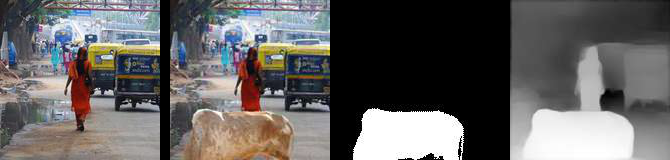
\includegraphics[width=1\textwidth]{samplerecord.png}
  \caption{Sample Record which contains the background image, a cow overlayed on top of background, its mask and depth images}
  \label{fig:samplerecord}
\end{figure}


\begin{figure}[h!]
\centering
  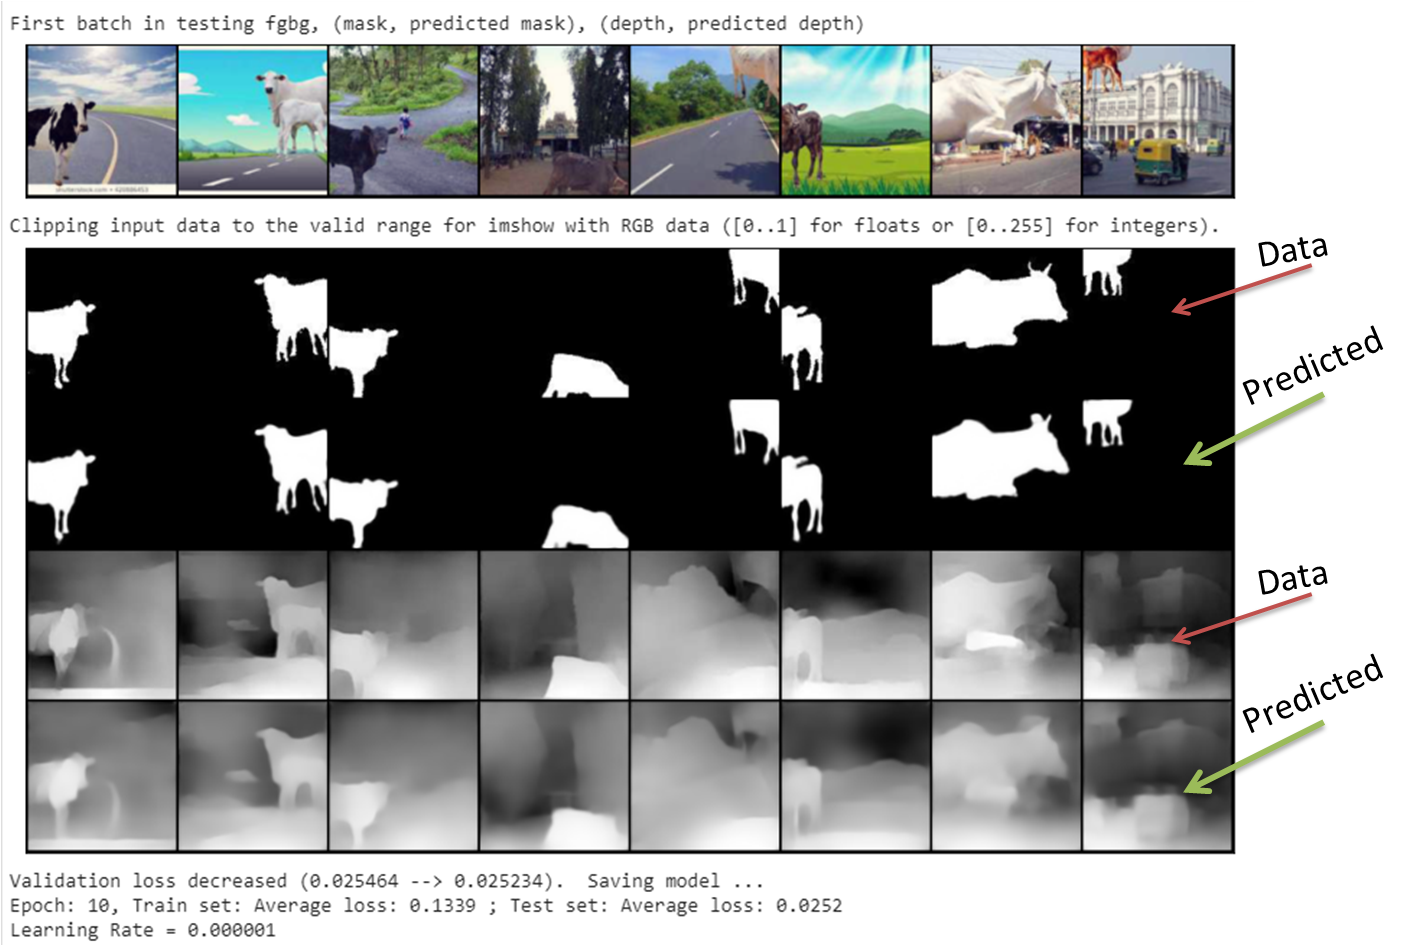
\includegraphics[width=1\textwidth]{finalepoch.png}
  \caption{Sample Record which contains the background image, a cow overlayed on top of background, its mask and depth images}
  \label{fig:samplerecord}
\end{figure}


\begin{figure}[h!]
\centering
  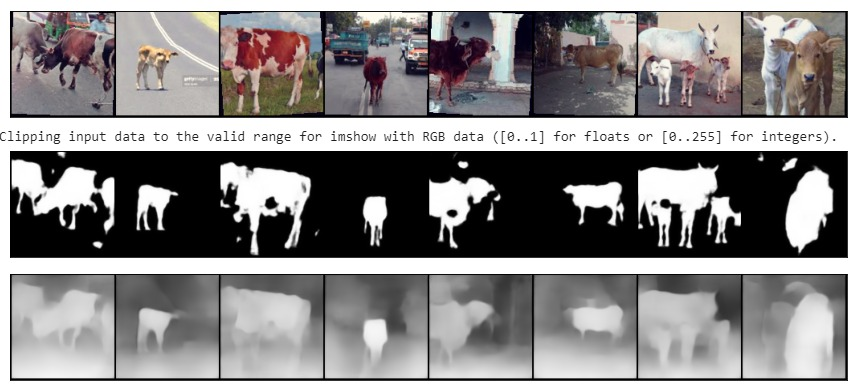
\includegraphics[width=1\textwidth]{unseen.jpeg}
  \caption{Sample Record which contains the background image, a cow overlayed on top of background, its mask and depth images}
  \label{fig:samplerecord}
\end{figure}


\section {Related Work}
[*** sentences need to be reframed with the help of Abhinav sir
A variety of RGBD datasets in which images are paired with corresponding depth maps(D) have been proposed through the years.
Available RGBD datasets
kitti dataset \cite{geiger2013vision}, the Synthia dataset \cite{ros2016synthia}, Make3D dataset \cite{saxena2008make3d}, NYU dataset \cite{silberman2012indoor}

It is the best known RGBD dataset collected using a vehicle equipped with a sparse Velodyne VLP-64 LiDAR scanner and RGB cameras, and features street scenes in and around the German city of Karlsruhe. Primary application of this dataset involves perception tasks in the context of self-driving.

Synthia is a street scene dataset with depth maps of synthetic data, requiring domain adaptiation to apply to real world settings. 

Cityscapes [reference] provides a dataset of street scenes, albeit with more diversity than KITTI.

Sintel [reference] is another synthetic dataset which includes outdorrs sences.

Megadepth [reference] is a large-scale dataset of outdoor internet images, with depth maps recon- structed using structure-from-motion techniques, but also lacking in ground truth depth and scale.

Make3D [reference] provides RGB and depth information for outdoor scenes

The NYUv2 dataset [reference] is widely used for monocular depth estimation in indoor environments. The data was col- lected with a Kinect RGBD camera, which provides sparse and noisy depth returns. These returns are generally in- painted and smoothed before they are used for monocular depth estimation tasks. As a result, while the dataset in- cludes sufficient samples to train modern machine learn- ing pipelines, the “ground-truth” depth does not necessarily correspond to true scene depth.
***]

\section{The XYZ dataset}
we designed the dataset with the following objectives...
1. dataset which dedicately include stray animals, as animals move without any restrictions in the small cities of India.
2. self driving cars should be able to identify animals
2. dataset should provide accurate dense depth maps.
4. dataset should provide foreground images

\subsection{Data Acquisition}
\subsection{Data Curation and Processing}
\subsection{Data Statistics}


\section{Experiments}
In this section, we provide a baseline for monocular depth estimation on the XYZ dataset
\subsection{Model}
\subsection{Evaluation}
\subsection{Analysis}

3. 
\section{Conclusion}
\section{Acknowledgement}
This paper and the research behind it would not have been possible without the exceptional support and computing facilities of my Institution, Vishnu Institute of Technology.
\begin{thebibliography}{10}
\bibitem{geiger2013vision} Geiger, Andreas, et al. "Vision meets robotics: The kitti dataset." The International Journal of Robotics Research 32.11 (2013): 1231-1237.

\bibitem{ros2016synthia} Ros, German, et al. "The synthia dataset: A large collection of synthetic images for semantic segmentation of urban scenes." Proceedings of the IEEE conference on computer vision and pattern recognition. 2016.

\bibitem{saxena2008make3d} Saxena, Ashutosh, Min Sun, and Andrew Y. Ng. "Make3D: Depth Perception from a Single Still Image." AAAI. Vol. 3. 2008.

\bibitem{silberman2012indoor} Silberman, Nathan, et al. "Indoor segmentation and support inference from rgbd images." European conference on computer vision. Springer, Berlin, Heidelberg, 2012.

\bibitem{marchand2015pose} Marchand, Eric, Hideaki Uchiyama, and Fabien Spindler. "Pose estimation for augmented reality: a hands-on survey." IEEE transactions on visualization and computer graphics 22.12 (2015): 2633-2651.

\end{thebibliography}
\end{document}
\section{Conclusion}
\section{Acknowledgement}
This paper and the research behind it would not have been possible without the exceptional support and computing facilities of my Institution, Vishnu Institute of Technology.
\begin{thebibliography}{10}



\end{thebibliography}
\end{document}